\begin{multicols}{2}
	\begin{center}
	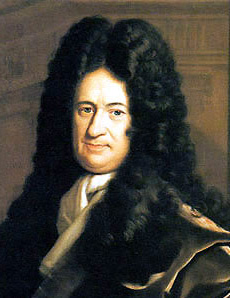
\includegraphics[height=.9\textheight]{./IMG/Gottfried+Wilhelm+Leibniz.jpg}
	\end{center}
	
	\vfill
	\columnbreak

\begin{itemize}
	\item séc. 18
	\item Lógica binária
	\item Escrituras chinesas
\end{itemize}	
\end{multicols}

\vfill
\pagebreak

\begin{center}
	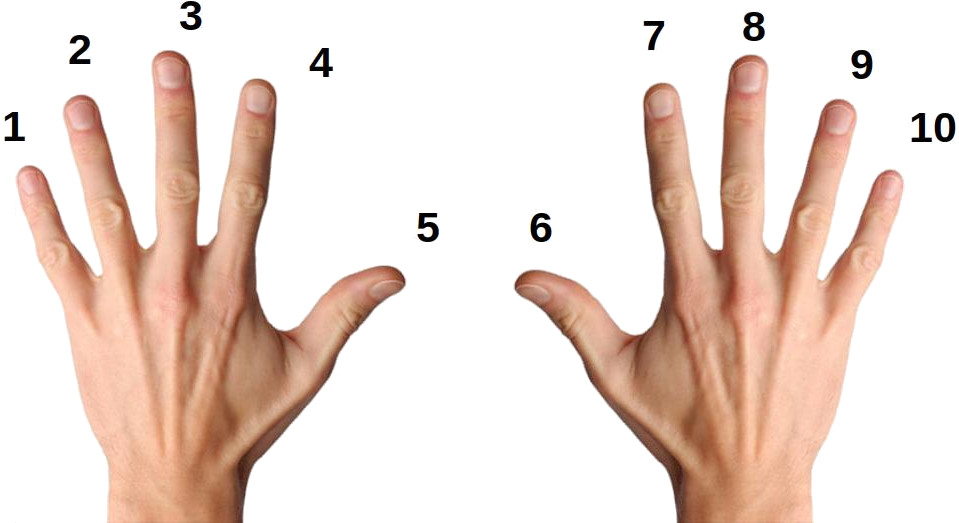
\includegraphics[height=\textheight]{./IMG/MAO-10.jpg}
\end{center}

\vfill
\pagebreak

{\Huge
Base 10
}
\vspace*{-10mm}
{
	\Large
\begin{center}
		\begin{tabular}{*{10}{r}}
	\csvreader[no head, tabular=*{9}{c}c, table head=\\]%
	{./CSV/TABELA.csv}{}%
	{\csvcoli &}%
\end{tabular}
\end{center}

}

\vfill
\pagebreak


\begin{multicols}{2}
	
	
	\begin{center}
		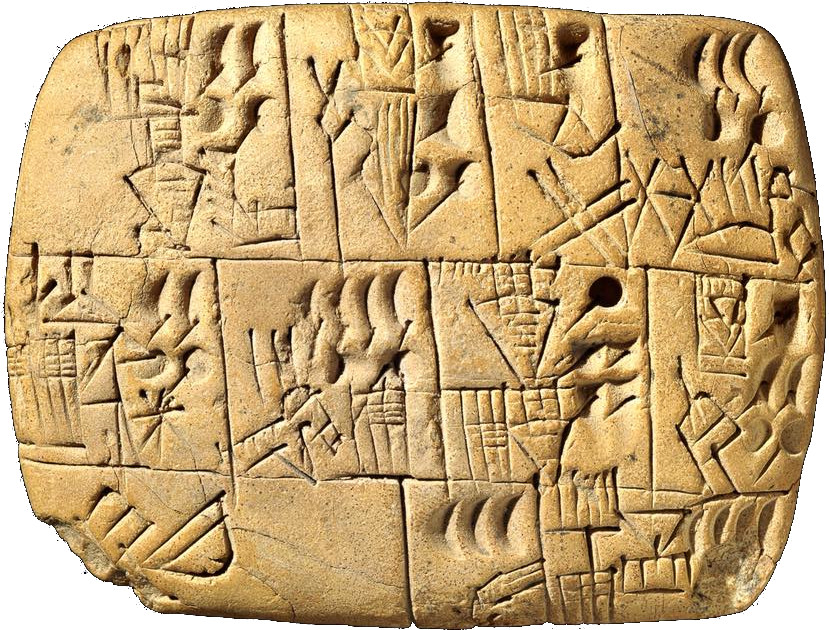
\includegraphics[width=\linewidth]{./IMG/argila.jpeg}
	\end{center}
	
	\vfill
	\columnbreak
	
	\begin{center}
	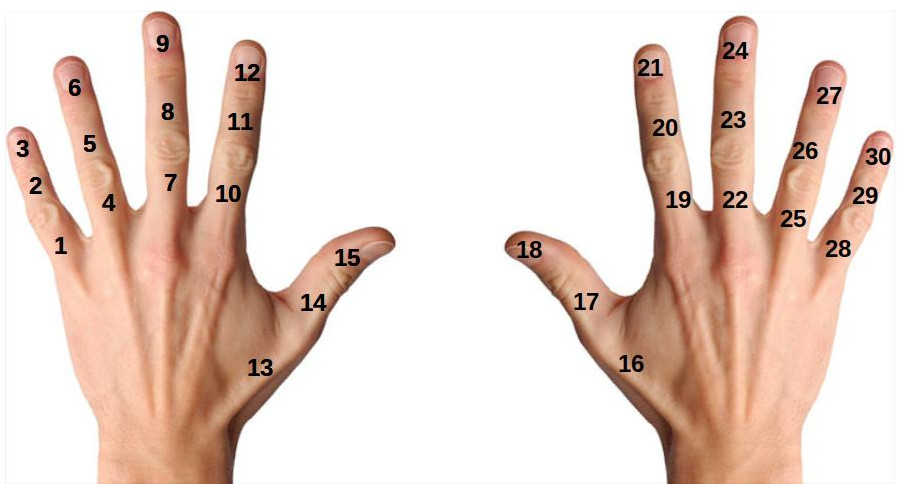
\includegraphics[height=.5\textheight]{./IMG/MAO-60.jpg}
	
	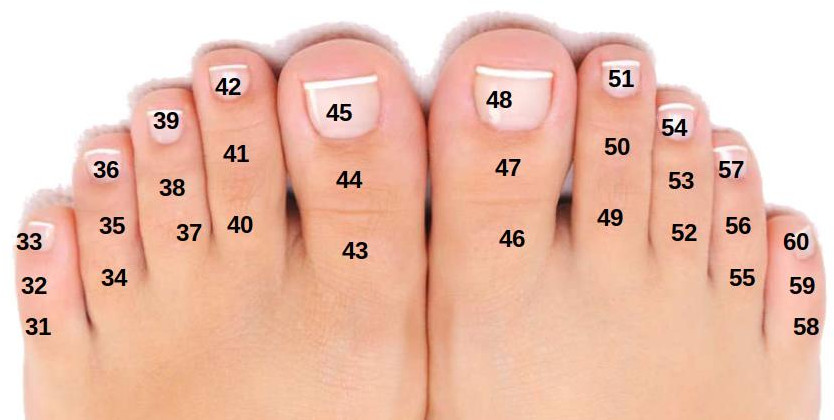
\includegraphics[height=.45\textheight]{./IMG/PES-60.jpg}
\end{center}
\end{multicols}

\vfill
\pagebreak

{\Huge
	Base 60
}
\begin{center}
	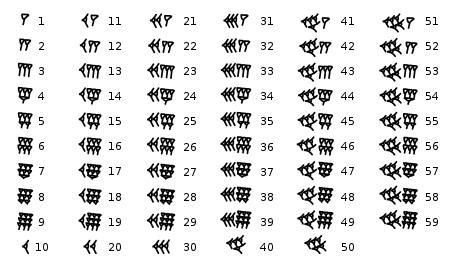
\includegraphics[height=.9\textheight]{./IMG/Babylonian_numerals.svg.png}
\end{center}

\vfill
\pagebreak

	\begin{center}
	
\includegraphics[height=\textheight]{./IMG/cobra.jpg}
\end{center}

\vfill
\pagebreak
\begin{multicols}{2}
	
	{\LARGE
		Base Binária: 0 e 1.
	}
	
	\large "[…] não uso nenhum outro caractere além do 0 e 1, e quando chego neste segundo, eu começo de novo."
	
	{\normalsize Fonte: \href{http://www.leibniz-translations.com/binary.htm}{http://www.leibniz-translations.com/binary.htm}}
	
	
%
\ExplSyntaxOn
\foreach \dec in {0,...,15} {%
	\int_to_bin:n { \dec } \\
}
\ExplSyntaxOff

%%
	\vfill\null
	\columnbreak
	




%	
%	\ExplSyntaxOn
%	\newsavebox{\mybox}
%	\begin{lrbox}{\mybox}
%		\begin{minipage}{\linewidth}
%			\begin{tabular}{|>{\raggedleft\arraybackslash}p{1.5cm}|>{\centering\arraybackslash}p{1.5cm}|}
%				\hline
%				\textbf{Decimal} & \textbf{Binário} \\
%				\hline
%				\foreach \dec in {0,...,15} {
%					\dec & \int_to_bin:n { \dec } \\
%					\hline
%				}
%			\end{tabular}
%		\end{minipage}
%	\end{lrbox}
%	
%	\noindent\usebox{\mybox}
%	\ExplSyntaxOff
%	
	
	
	

%\newsavebox{\mybox}
%\begin{lrbox}{\mybox}
%	\begin{minipage}{\linewidth}
%		\begin{tabular}{|>{\raggedleft\arraybackslash}p{1.5cm}|>{\centering\arraybackslash}p{1.5cm}|}
%			\hline
%			\textbf{Decimal} & \textbf{Binário} \\
%			\hline
%			\ExplSyntaxOn
%			\foreach \dec in {0,...,15} {
%				\dec & \int_to_bin:n { \dec } \\
%				\hline
%			}
%			\ExplSyntaxOff
%		\end{tabular}
%	\end{minipage}
%\end{lrbox}
%
%\begin{tabular}{p{\linewidth}}
%	\usebox{\mybox}
%\end{tabular}

		\vfill
	\columnbreak
\normalsize	
%
%\begin{flushright}
%\textbf{	\begin{tabular*}{\textwidth}{@{\extracolsep{\fill}}*{3}{r}@{}}
%	\csvreader[no head, tabular=*{2}{r}r, table head=\\]%
%		{./CSV/BINARIOS.csv}{}%
%		{\csvcoli & \csvcolii & \csvcoliii}%
%	\end{tabular*}}
%\end{flushright}

\end{multicols}

\vfill
\pagebreak
{\LARGE 4 operações}
\begin{center}
	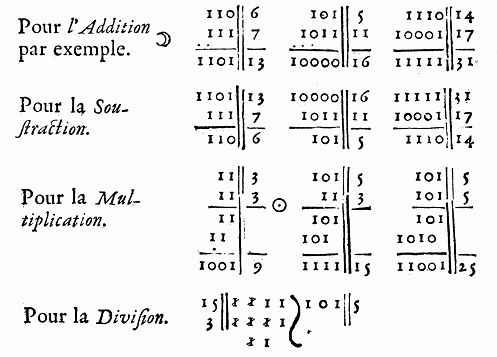
\includegraphics[height=.9\textheight]{./IMG/leibnizbinario.png}
\end{center}

\vfill
\pagebreak